\documentclass[12pt,a4paper]{article}
\usepackage[margin=23mm,top=24mm,bottom=23mm]{geometry}
\usepackage{fontspec,amsmath,amssymb,booktabs,graphicx,xcolor,fancyhdr,hyperref}
\usepackage{tikz}
\setmainfont{TeX Gyre Pagella}
\setsansfont{TeX Gyre Heros}
\setmonofont{Latin Modern Mono}[Scale=0.87]
\linespread{1.06}
\definecolor{ink}{HTML}{193A52}
\definecolor{teal}{HTML}{00696B}
\hypersetup{colorlinks=true,linkcolor=teal,urlcolor=teal,pdftitle={TiSe2: DFT fononi pri zadanoj elektronskoj temperaturi}}
\setlength{\parindent}{0pt}\setlength{\parskip}{5.5pt}
\setlength{\emergencystretch}{3em}
\pagestyle{fancy}\fancyhf{}
\fancyhead[L]{\sffamily\small MRMFKT \quad Materijali za projekt}
\fancyhead[R]{\sffamily\small Monosloj 1T-TiSe$_2$}
\fancyfoot[R]{\sffamily\small\thepage}
\newcommand{\sect}[1]{\vspace{4pt}\noindent{\large\sffamily\bfseries\color{ink}#1}\par}
\newcommand{\titlepagepart}[1]{{\fontsize{23}{28}\selectfont\sffamily\bfseries\color{ink}#1}\par\vspace{3pt}}
\newcommand{\code}[1]{\texttt{\detokenize{#1}}}
\newcommand{\qe}{Quantum ESPRESSO}
\begin{document}
\titlepagepart{Što se mijenja kada zagrijemo elektrone?}
U prvom dijelu projekta pomaknuli smo atome i pitali MACE kolike su sile. Sada za zadane položaje atoma rješavamo elektronski problem u DFT-u. Možemo promijeniti zaposjednutost elektronskih stanja i ponovno pitati koliko je strukturu lako deformirati. Upravo tu mogućnost koristi drugi dio zadatka.

\sect{Jedna temperatura, dvije geometrije}
Krećemo od visokosimetričnog monosloja s jednim Ti i dva Se u primitivnoj ćeliji. Najprije određujemo ravnotežnu visinu Se iznad i ispod ravnine Ti pri zadanoj elektronskoj temperaturi \(T_e\). Računamo disperziju te strukture. Zatim uzimamo četiri kopije ćelije, ukupno 12 atoma. Na toj većoj ćeliji postavljamo dva pitanja.

\begin{tabular}{@{}p{0.28\linewidth}p{0.65\linewidth}@{}}
\toprule
\textbf{Simetrična struktura} & Koliko se energija promijeni duž jednog M-moda? Što dobijemo ako zajedno pobudimo tri ekvivalentna M-moda? U obje usporedbe polazimo od istih 12 položaja.\\[3pt]
\textbf{Relaksirana struktura} & Kamo će atomi otići ako im dopustimo da se svi pomiču? Daje novu geometriju i vlastiti skup fonona oko nje.\\
\bottomrule
\end{tabular}

\sect{Kako temperatura ulazi u račun}
Kao u primjeru za metalni Ni s vježbe 5, koristimo razmazivanje zaposjednutosti oko Fermijeve energije. Za ovaj zadatak biramo Fermi--Diracovu funkciju \(f(\epsilon)=1/[1+\exp((\epsilon-\mu)/k_BT_e)]\). U \code{pw.x} pišemo \code{occupations='smearing'}, \code{smearing='fd'} i širinu \code{degauss} u rydberzima. Primjer za 400 K daje \(k_BT_e=0{,}03447\) eV, odnosno \(0{,}00253345\) Ry.

\begin{center}\begin{tabular}{rrrrrrr}\toprule
\(T_e\) (K) & 100 & 200 & 400 & 800 & 1200 & 1600\\
\code{degauss} (Ry) & .00063336 & .00126672 & .00253345 & .00506690 & .00760035 & .01013380\\
\bottomrule\end{tabular}\end{center}
Račun za svaku geometriju daje elektronsku slobodnu energiju \(F=E-T_eS_{\rm el}\). U ispisu \code{pw.x} koristimo završni redak \code{! total energy} koji za ovaj izbor već sadrži entropijski doprinos. Ioni se u relaksaciji pomiču po silama do stacionarne geometrije. Njihovo toplinsko gibanje ovim postupkom ne simuliramo.

\newpage
\titlepagepart{Od sile na atomu do disperzije}
\sect{Zašto prvo relaksiramo}
U vježbi 2 vidjeli smo \(F_i=-\partial E/\partial R_i\) i tražili mjesto gdje sile iščezavaju. Isti BFGS postupak ovdje koristi DFT sile. U primitivnoj ćeliji držimo \(a=3{,}54\) Å radi usporedbe s prvim dijelom projekta. Ti određuje ishodište, a Se se mogu relaksirati po \(z\). Simetrija roditeljske strukture čuva se u toj ćeliji. Iščezavanje sila govori o prvoj derivaciji. Stabilnost zahtijeva i podatak o drugoj derivaciji.

U našem dovršenom računu pri 100 K visina Se promijenila se s 1,55000 na 1,55215 Å. Nakon četiri koraka BFGS-a najveća je sila bila \(1{,}70\times10^{-5}\) eV/Å. Te podatke možeš provjeriti u \code{T0100K/relax_1x1/relax.out}. Za fiksni \(a\) dobili smo \(\sigma^{2D}_{xx}=\sigma^{2D}_{yy}=-5{,}09\times10^{-4}\) eV/Ų prema istoj konvenciji kao u našoj bilježnici. Odgovarajuća tablica je \code{naprezanje_2d.csv}.

\sect{Što program zapravo dijagonalizira}
Na predavanju 6 iz malog pomaka iona izveli smo odziv elektronske gustoće, zatim konstante sila \(\Phi=\partial^2 F/\partial u\,\partial u\). U vježbi 4 taj se odnos procjenjivao pomicanjem atoma i razlikama sila. Ovdje \code{ph.x} računa isti harmonijski objekt linearnim odzivom (DFPT). Fourierovom transformacijom po ćelijama i dijeljenjem masama dobivamo dinamičku matricu. Za svaki valni vektor rješavamo
\[
 D(\mathbf q)e_{\mathbf q j}=\omega_{\mathbf q j}^2e_{\mathbf q j},\qquad
 \nu=\omega/(2\pi).
\]
Tri atoma daju devet grana. Negativna svojstvena vrijednost znači negativnu zakrivljenost i imaginarni \(\omega\). Na grafu crtamo \(-|\nu|\) za takav mod. Vrijedi pročitati i oznaku osi jer je jedinica THz frekvencija. Malen negativan broj blizu akustičke nule u \(\Gamma\) treba provjeriti na gušćoj mreži prije fizičkog tumačenja.

\sect{Kako nastaje linija \(\Gamma\)--M--K--\(\Gamma\)}
\code{pw.x} daje samosuglasnu elektronsku gustoću. \code{ph.x} potom računa odziv na mreži \(6\times6\times1\) fononskih \(\mathbf q\)-točaka. Po uzoru na primjer za MgO s vježbe 6, \code{q2r.x} pretvara te matrice u konstante sila u realnom prostoru, a \code{matdyn.x} ih interpolira duž putanje. Elektronska \(\mathbf k\)-mreža služi integraciji elektronskih stanja. Fononska \(\mathbf q\)-mreža određuje valne duljine deformacija koje izravno uzorkujemo.

U našoj recipročnoj bazi vrijedi \(\Gamma=(0,0,0)\), \(\mathrm M=(1/2,0,0)\) i \(\mathrm K=(1/3,1/3,0)\). M se nalazi na odabranoj mreži. Uz minimum cijele putanje spremamo i minimum točno u M. Kao neovisnu provjeru zadajemo i izravan DFPT račun samo u M. \code{ph.x} za taj pojedinačni unos očekuje kartezijske komponente u jedinicama \(2\pi/a\), pa ulaz glasi \((1/2,1/(2\sqrt3),0)\).

U prvom dijelu MACE-PBE dao je oko \(-4{,}11\) THz u M. S DFT-om prvo usporedi položaj nestabilnosti, zatim veličinu imaginarne frekvencije i obrazac pomaka. DFT i MACE imaju različita ishodišta apsolutne energije pa potencijale uspoređuj preko \(\Delta F(A)\).

\newpage
\titlepagepart{Zašto se nestabilnost iz M vidi u \(\Gamma\)?}
Za mod \(\mathbf M_1=(1/2,0,0)\) susjedna primitivna ćelija u smjeru \(\mathbf a_1\) dobiva fazu \(\exp(i\pi)=-1\). Nakon dvije takve translacije faza opet postaje \(+1\). Cijeli uzorak zato stane unutar jedne superćelije 2×2 i ponavlja se od superćelije do superćelije. U njezinoj Brillouinovoj zoni ima \(\mathbf q=\Gamma\). To je isto savijanje zone koje smo vidjeli za konvencionalnu ćeliju Cu na vježbi 4.

\begin{center}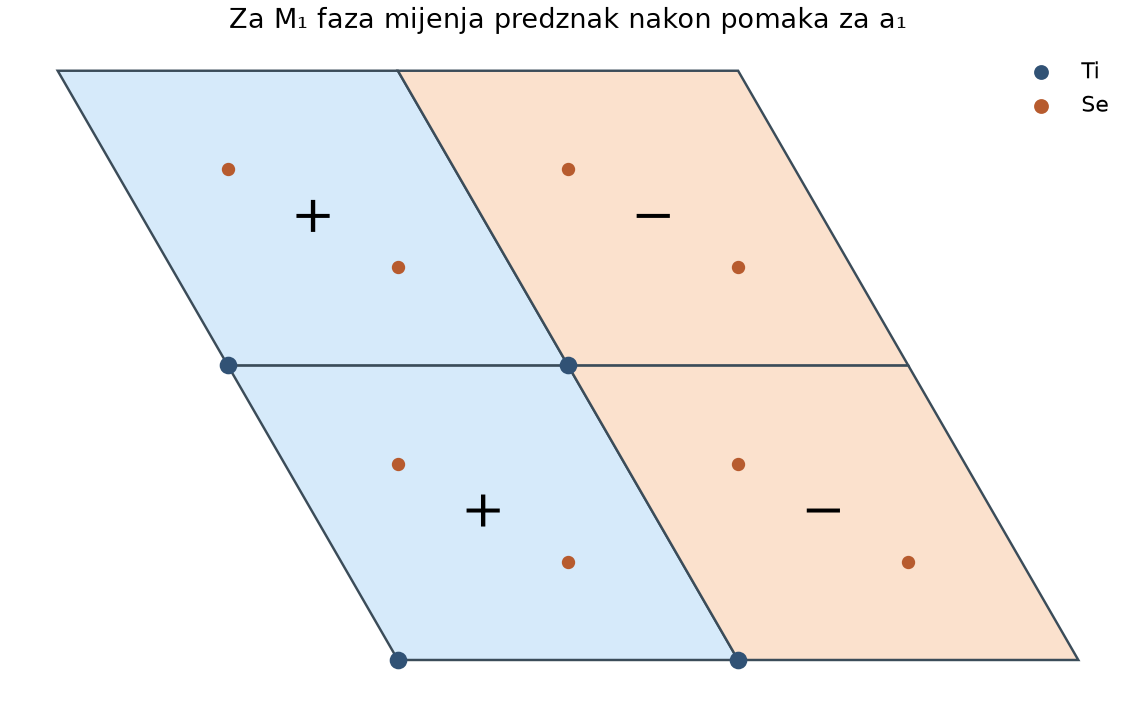
\includegraphics[width=.77\linewidth]{slike/faza_M1.png}\end{center}
Na slici znak označava fazu uzorka pomaka u svakoj kopiji. Smjer i veličinu pomaka pojedinih atoma tek daje DFT svojstveni vektor. Dva sloja Se prikazana su u projekciji odozgo.

\sect{Kako iz 36 modova odabrati pravi}
Za visokosimetričnu superćeliju računamo samo odziv u \(\Gamma\), kao u primjeru za Si s vježbe 6. Dvanaest atoma daje 36 modova. U toj se točki sastaju četiri sektora iz primitivne zone, \(\Gamma,\mathrm M_1,\mathrm M_2,\mathrm M_3\), svaki s devet stupnjeva slobode. Dijagonalizator smije miješati svojstvene vektore iste frekvencije. Za njihovo razdvajanje koristimo predznake po četirima kopijama, poredanima kao \((0,0),(0,1),(1,0),(1,1)\).

\begin{center}\begin{tabular}{@{}lcr@{}}\toprule
Sektor & \(\mathbf q\) u primitivnoj recipročnoj bazi & Znakovi kopija\\\midrule
\(\mathrm M_1\) & \((1/2,0,0)\) & \(+,+,-,-\)\\
\(\mathrm M_2\) & \((0,1/2,0)\) & \(+,-,+,-\)\\
\(\mathrm M_3\) & \((1/2,-1/2,0)\) & \(+,-,-,+\)\\\bottomrule
\end{tabular}\end{center}
Za svaki red konstruiramo matricu \(B\) tako da tri atomska pomaka primitivne ćelije kopiramo s navedenim znakovima i faktorom \(1/2\). Dijagonaliziramo \(B^\mathsf{T} D B\) veličine \(9\times9\), odaberemo granu pa se s \(e=Bv\) vratimo na svih 36 komponenti. Za M$_3$ izbor \(+1/2\) umjesto \(-1/2\) na drugoj koordinati daje iste znakove. Datoteka \code{nestabilni_vektori.csv} sadrži i sve izvorne nestabilne smjerove pune dijagonalizacije.

\newpage
\titlepagepart{Što si zbrojio u bilježnici?}
Redak \code{u = mod1["u"] + mod2["u"] + mod3["u"]} zbraja tri uzorka pomaka \emph{za isti atom}. Kod četiri atoma Ti vidiš da tri rezultantne strelice pokazuju u različitim smjerovima, dok se četvrtom doprinosi poništavaju. Svi se pomaci množe istim brojem, pa put kroz prostor 36 koordinata i dalje ima samo jednu slobodnu amplitudu.

\begin{center}
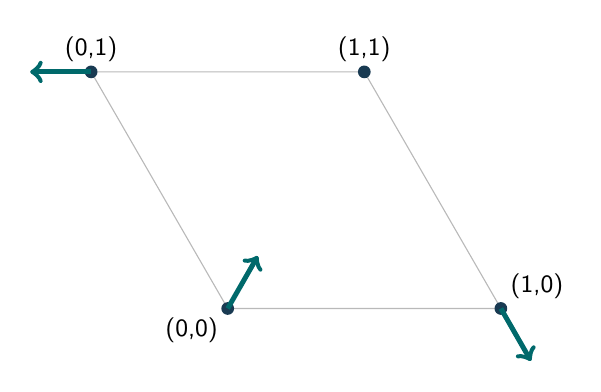
\begin{tikzpicture}[x=0.98cm,y=0.98cm,every node/.style={font=\small\sffamily}]
  \draw[gray!55] (0,0)--(3.54,0)--(1.77,3.066)--(-1.77,3.066)--cycle;
  \foreach \x/\y in {0/0,3.54/0,1.77/3.066,-1.77/3.066}{\fill[ink] (\x,\y) circle (2.3pt);}
  \draw[->,teal,line width=1.8pt] (0,0)--(.39,.68);
  \draw[->,teal,line width=1.8pt] (-1.77,3.066)--(-2.56,3.066);
  \draw[->,teal,line width=1.8pt] (3.54,0)--(3.93,-.68);
  \node[below left] at (0,0) {(0,0)};
  \node[above] at (-1.77,3.07) {(0,1)};
  \node[above right] at (3.54,0) {(1,0)};
  \node[above] at (1.77,3.07) {(1,1)};
\end{tikzpicture}
\end{center}
{\small Četiri Ti u prikazu odozgo. Strelice daju relativne smjerove iz tvoje tablice za MACE-PBE. U računu energije sudjeluje i svih osam atoma Se.}

\sect{Što je na osi grafa?}
Fononska disperzija prikazuje frekvenciju prema valnom vektoru \(\mathbf q\). Tvoj novi graf prikazuje \(\Delta E\) prema \emph{amplitudi} na putu kroz istu visokosimetričnu strukturu. Promijenio si smjer u kojem ispituješ energiju. Za novu fononsku disperziju trebalo bi ponovno računati druge derivacije oko odabrane nove geometrije.

\begin{center}\begin{tabular}{@{}llrr@{}}\toprule
MACE model & Presjek & \(\lvert A_\mathrm{min}\rvert\) (Å) & \(E(0)-E_\mathrm{min}\) (meV/2×2)\\\midrule
PBE & samo M$_1$ & 0,056 & 11,1886\\
PBE & tri M-moda & 0,084 & 19,3714\\
r$^2$SCAN & samo M$_1$ & 0,048 & 9,6650\\
r$^2$SCAN & tri M-moda & 0,072 & 16,5313\\\bottomrule
\end{tabular}\end{center}
To su minimumi na mreži iz spremljenih MACE ispisa u bilježnici. Na oba presjeka obje strane u tim ispisima imaju istu dubinu do prikazane preciznosti. Za DFT se svaki unos zasebno izračunava pri njegovu \(T_e\). Tri pojedinačna obrasca i njihovu vezu s distorzijom vala gustoće naboja možeš usporediti sa slikom 6 u radu \href{https://ddd.uab.cat/pub/artpub/2018/195676/2dmaterials_a2018v5n2p025024.pdf}{Guster i sur., \emph{2D Materials} (2018)}.

\newpage
\titlepagepart{Kako usporediti dvije amplitude?}
\sect{Od maseno ponderiranog vektora do položaja u Å}
Neka su \(e_1,e_2,e_3\) međusobno ortogonalni, jedinični vektori triju sektora. Na 100 K biramo najnižu granu u svakom sektoru i postavljamo predznak kao u bilježnici: komponenta najvećeg iznosa u prvoj primitivnoj kopiji je pozitivna. Na sljedećoj temperaturi biramo najveći apsolutni preklop zasebno u svakom sektoru i uskladimo predznak. Time izbor \((+,+,+)\) dobiva ponovljivo značenje.
\[
 e_{\mathrm{1Q}}=e_1,\qquad
 e_{\mathrm{3Q}}=(e_1+e_2+e_3)/\sqrt3,\qquad
 w_i=e_i/\sqrt{m_i},\qquad
 \mathbf R_i(Q)=\mathbf R_i(0)+Qw_i .
\]
Ovdje je \(e_i\) trokomponentni dio \emph{odabranog} vektora na atomu \(i\). Za oba smjera vrijedi \(\sum_i m_i|w_i|^2=1\). Na zajedničkoj osi crtamo \(A=Q\max_i |w_i|\), u Å. Pri \(A=0{,}03\) Å najviše pomaknuti atom u oba pokusa prijeđe 0,03 Å.

U tvojem kodu tri su pomaka zbrojena prije normiranja, pa je njihov maseno ponderirani iznos \(\sqrt3\). Za iste položaje vrijedi \(Q_{\mathrm{3Q}}=\sqrt3\,Q_{\rm bilježnica}\). Primjerice, \(\lvert Q_{\rm bilježnica}\rvert=0{,}6650\) u PBE minimumu znači \(\lvert Q_{\mathrm{3Q}}\rvert\simeq1{,}152\) Å\(\sqrt{\rm amu}\); fizički pomak ostaje 0,084 Å. U kodu svaki \code{smjer_*.csv} daje \(e_i\), \(w_i\) i \(w_i/\max_j|w_j|\).

\sect{Koja parabola pripada zbroju?}
U maseno ponderiranim koordinatama i odgovarajućim energetskim jedinicama harmonijski član glasi
\[
 \Delta F_{\rm harm}(Q)=\tfrac12\kappa Q^2,\qquad
 \kappa=e^\mathsf{T}De.
\]
Za simetričnu 2×2 ćeliju tri sektora su ortogonalna i ne miješaju se. Za jedinični 3Q smjer tada je \(\kappa=(\lambda_1+\lambda_2+\lambda_3)/3\). Na tvojoj izvornoj osi za nenormirani zbroj koeficijent uz \(Q_{\rm bilježnica}^2/2\) jest \(\lambda_1+\lambda_2+\lambda_3\). Pri točnoj degeneraciji to je \(3\lambda_1\). Stoga u ćeliji 9.1 stara parabola s jednom \(\lambda_1\) odgovara jedno-modnom presjeku.

U kodu matrica ima svojstvene vrijednosti \(\nu|\nu|\) u THz², gdje je \(\nu\) predznačena frekvencija iz QE-a. Pri pretvorbi projekcije u eV/Ų za os \(A\) kod uključuje faktor \((2\pi)^2\) i efektivnu masu smjera. Zapisuje i \(\|De-\kappa e\|\) u jedinicama matrice. Pri degeneraciji je i zbroj svojstveni vektor. Pri razdvojenim vrijednostima presjek ima smisao kao put sa svojom projiciranom zakrivljenošću.

\newpage
\titlepagepart{Presjek energije i novi minimum}
\sect{Što točno mjeri svaki DFT presjek?}
Od iste visokosimetrične strukture pri istom \(T_e\) krećemo jednom duž M$_1$, drugi put duž 3Q. Za svaki nenulti \(A\) radimo novi elektronski SCF pri zamrznutim ionskim položajima. Zadanih 13 amplituda svakog smjera pokriva od \(-0{,}16\) do \(+0{,}16\) Å. Oba presjeka dijele već izračunatu referencu \(F(0,T_e)\) i zahtijevaju ukupno 24 dodatna SCF računa po temperaturi. U bilježnici je razmak bio 0,004 Å. DFT tablice zato mogu dati drukčiji položaj minimuma već zbog rjeđe mreže pomaka.

Na osi energije je \(\Delta F(A)=F(A,T_e)-F(0,T_e)\) u meV po superćeliji. Dijeljenjem s četiri dobiva se meV po formulskoj jedinki TiSe$_2$. Kod negativne zakrivljenosti mali pomak spušta energiju. Za M$_1$ translacija za \(\mathbf a_1\) zamjenjuje \(+A\) i \(-A\). Iz tablice znakova vidiš da nijedna primitivna translacija ne obrće sva tri M-moda odjednom. Obje strane 3Q zato računamo izravno; moguće slaganje može biti posljedica drugih simetrija. Kontrola \([F(h)+F(-h)-2F(0)]/h^2\) pri \(h=0{,}01\) Å uspoređuje energije s DFPT-om. Ako je najmanja vrijednost na rubu intervala, dubina dobivena na mreži još ne određuje položaj jame.

\sect{Što dopušta slobodna relaksacija 2×2}
Svim atomima dodajemo malu slučajnu distorziju, uklonimo translaciju centra mase i postavimo korijen srednjeg kvadrata veličine pomaka na \(0{,}03\) Å. Svi \(T_e\) kreću od istog uzorka šuma kako bi usporedba bila ponovljiva. BFGS sada smije mijenjati sve atomske koordinate. Tako može nastati kombinacija više M-modova koju jednim presjekom nismo mogli istražiti. Jedan slučajni početak može dati lokalni minimum. Promjena \code{random_seed} omogućuje ponavljanje s drugim početkom.

Nakon konvergencije ponovno radimo SCF i DFPT u \(\Gamma\) \emph{nove} strukture. Provjeravamo jesu li ostale imaginarne frekvencije. Pomaknu li se dva moda dovoljno da promijene redoslijed, “četvrta frekvencija” na različitim temperaturama može pripadati različitim uzorcima gibanja. Zato izuzimamo tri translacije pa uparujemo ostala 33 vektora susjednih temperatura preko \(\lvert e_i^\mathsf T e_j\rvert^2\).

Na grafu ističemo granu s najvećim rasponom predznačene frekvencije. Za svaki mod spremamo preklop s jednom 3Q kombinacijom i ukupni udio u sva tri M-smjera. Prvi ovisi o relativnim predznacima i domeni, a drugi je zbroj triju kvadrata preklopa. U \code{distorzija_M.csv} statički pomak relaksirane strukture rastavljamo na tri M-komponente. Time možeš provjeriti jesu li se nakon slobodne relaksacije doista pojavile sve tri. Bliska degeneracija i malen preklop s prethodnom temperaturom traže pregled vektora prije imenovanja grane.

\newpage
\titlepagepart{Kako čitati rezultate i provjeriti zaključak}
\sect{Numerički izbori}
Polazni račun koristi PBE, skalarno-relativističke PAW pseudopotencijale PSLibrary s Ti polujezgrenim stanjima, odsječenja 60/600 Ry za valne funkcije i gustoću te mrežu \(24\times24\times1\) za primitivnu ćeliju. U 2×2 mreža je \(12\times12\times1\) pa je gustoća elektronskih točaka jednaka. Simuliramo ponovljenu neutralnu ploču u trodimenzionalnom periodičnom QE okviru s \(c=23{,}1052\) Å. Između susjednih ploča ima oko 20 Å praznog prostora. Visina ćelije i ravninski parametar fiksni su na svim temperaturama.

Širina na 100 K iznosi samo 8,62 meV. Vrijedi utvrditi koliko se frekvencija u M mijenja s elektronskom mrežom. \code{konvergencija.py} ponavlja izravan račun u M za \(k=24,36,48\) i odvojeno mijenja odsječenja i visinu ćelije. Za oblik između izravnih \(\mathbf q\)-točaka povećaj i fononsku mrežu, primjerice na \(8\times8\times1\) uz kompatibilnu \(k\)-mrežu. Prag 0,05 THz služi označavanju modova u tablicama. Procjenu stvarne pogreške daju usporedbe mreža. Najosjetljivije su temperature gdje \(\nu^2\) prolazi blizu nule.

\sect{Datoteke za pregled}
\begin{tabular}{@{}p{.42\linewidth}p{.52\linewidth}@{}}
\toprule
\code{status.csv} & Dovršenost svake faze na svakoj temperaturi.\\
\code{disperzija_0100K.png} & Devet grana. Svaka temperatura ima vlastiti graf.\\
\code{usporedba.csv} & M iz putanje, izravan M, presavijeni M te energija relaksacije 2×2.\\
\code{M_triplet_prema_T.csv} & Frekvencije sva tri M-moda, njihovo razdvajanje i 3Q zakrivljenost.\\
\code{PES_usporedba.csv} & Dubine oba presjeka, asimetrija i provjera zakrivljenosti.\\
\code{PES_M1_3Q_0100K.png} & Oba presjeka na istoj skali pomaka, za 100 K.\\
\code{grane_relaksirane.csv} & Frekvencije, preklopi i degeneracije kroz temperature.\\
\bottomrule
\end{tabular}

Kod ne pretpostavlja da će prijelaz nastupiti između 100 i 1600 K. Promjenu znaka \(\nu^2_\mathrm M\) možemo smjestiti između dvije izračunate temperature ako je znak numerički robustan. Elektronsko razmazivanje u ovom harmonijskom eksperimentu samo po sebi ne određuje eksperimentalnu temperaturu faznog prijelaza.

\sect{Veza s materijalima kolegija i izvorima}
\code{vjezbe2.ipynb} povezuje silu, zakrivljenost i optimizaciju. \code{vjezbe4.ipynb} izvodi fononske grane i savijanje zone. \code{vjezbe5.zip} sadrži SCF za Ni i relaksaciju za Si.

U vježbi 6 usporedi \code{01_Si_Gamma/ph.in} i \code{03_MgO_disp/ph_mesh.in}. Za izvod DFPT-a otvori \code{dfpt_fundamentals.pdf} iz mape \code{predavanje6} i pročitaj odjeljak 7.

\href{https://www.quantum-espresso.org/Doc/INPUT_PW.html}{QE: elektronski ulaz}\quad
\href{https://www.quantum-espresso.org/Doc/INPUT_PH.html}{DFPT}\quad
\href{https://www.quantum-espresso.org/Doc/INPUT_MATDYN.html}{Interpolacija}\quad
\href{https://www.quantum-espresso.org/Doc/INPUT_DYNMAT.html}{Svojstveni vektori}\quad
\href{https://pseudopotentials.quantum-espresso.org/}{Pseudopotencijali}

\newpage
\titlepagepart{Kako pokrenuti račun}
Otvori PowerShell u mapi projekta \code{MRMFKT}. Uđi u mapu DFT dijela i odaberi interpreter iz istog virtualnog okruženja koje koristi bilježnica.
\begin{verbatim}
cd DFT_TiSe2
$py = "..\.venv\Scripts\python.exe"
& $py studija.py status
\end{verbatim}
\sect{Jedna temperatura za čitanje korak po korak}
\begin{verbatim}
& $py studija.py run --temperatures 100 --part mesh
& $py studija.py run --temperatures 100 --part ref
& $py studija.py run --temperatures 100 --part pes
& $py studija.py run --temperatures 100 --part rel
\end{verbatim}
\begin{enumerate}\raggedright
\item \code{mesh} najprije relaksira primitivnu ćeliju. Otvori njezinu disperziju pa provjeri gdje najniža grana ulazi ispod nule. \code{--part m} daje i neovisni izravni račun točno u M.
\item \code{ref} izdvaja tri M-vektora u \(\Gamma\) simetrične 2×2. Otvori \code{smjerovi_M.json} pod \code{gamma_2x2_ref}. Usporedi tri frekvencije i 3Q rezidual. U mapi rezultata slike \code{pomaci_M1_0100K.png} i \code{pomaci_3Q_0100K.png} prikazuju strelice na istih 12 atoma.
\item \code{pes} sprema po jedan \code{potencijal.csv} pod \code{pes/M1} i \code{pes/3Q}. Na slici \code{PES_M1_3Q_0100K.png} usporedi dubinu i položaj minimuma po istoj apscisi \(A\). Zatim otvori \code{zakrivljenost.json} za svaki presjek.
\item \code{rel} počinje od slučajno narušene ćelije i daje spektar oko relaksiranih položaja. Nakon više temperatura u \code{najveci_pomak.json} pronađi granu najvećeg raspona i prati njezin redak u \code{grane_relaksirane.csv}.
\end{enumerate}
\sect{Svih šest temperatura}
\begin{verbatim}
& $py studija.py run
& $py studija.py report
\end{verbatim}
Naredba \code{run} uključuje i izravni M. Već potvrđeni koraci iste konfiguracije mogu se iskoristiti pri nastavku. \code{report} osvježava prikaze iz postojećih izlaza. Za zadane postavke zajedničke su tablice i slike u \code{racuni/k24_q6_17503ad3bf/rezultati/}. Postupak instalacije na drugom računalu i opcija dviju istodobnih grana nalaze se u \code{README.md}.
\end{document}
